\section{Clustering Pipeline} \label{sec:Clustering_Pipeline}

\blindtext

\begin{figure}[!hbt]
    \centering
    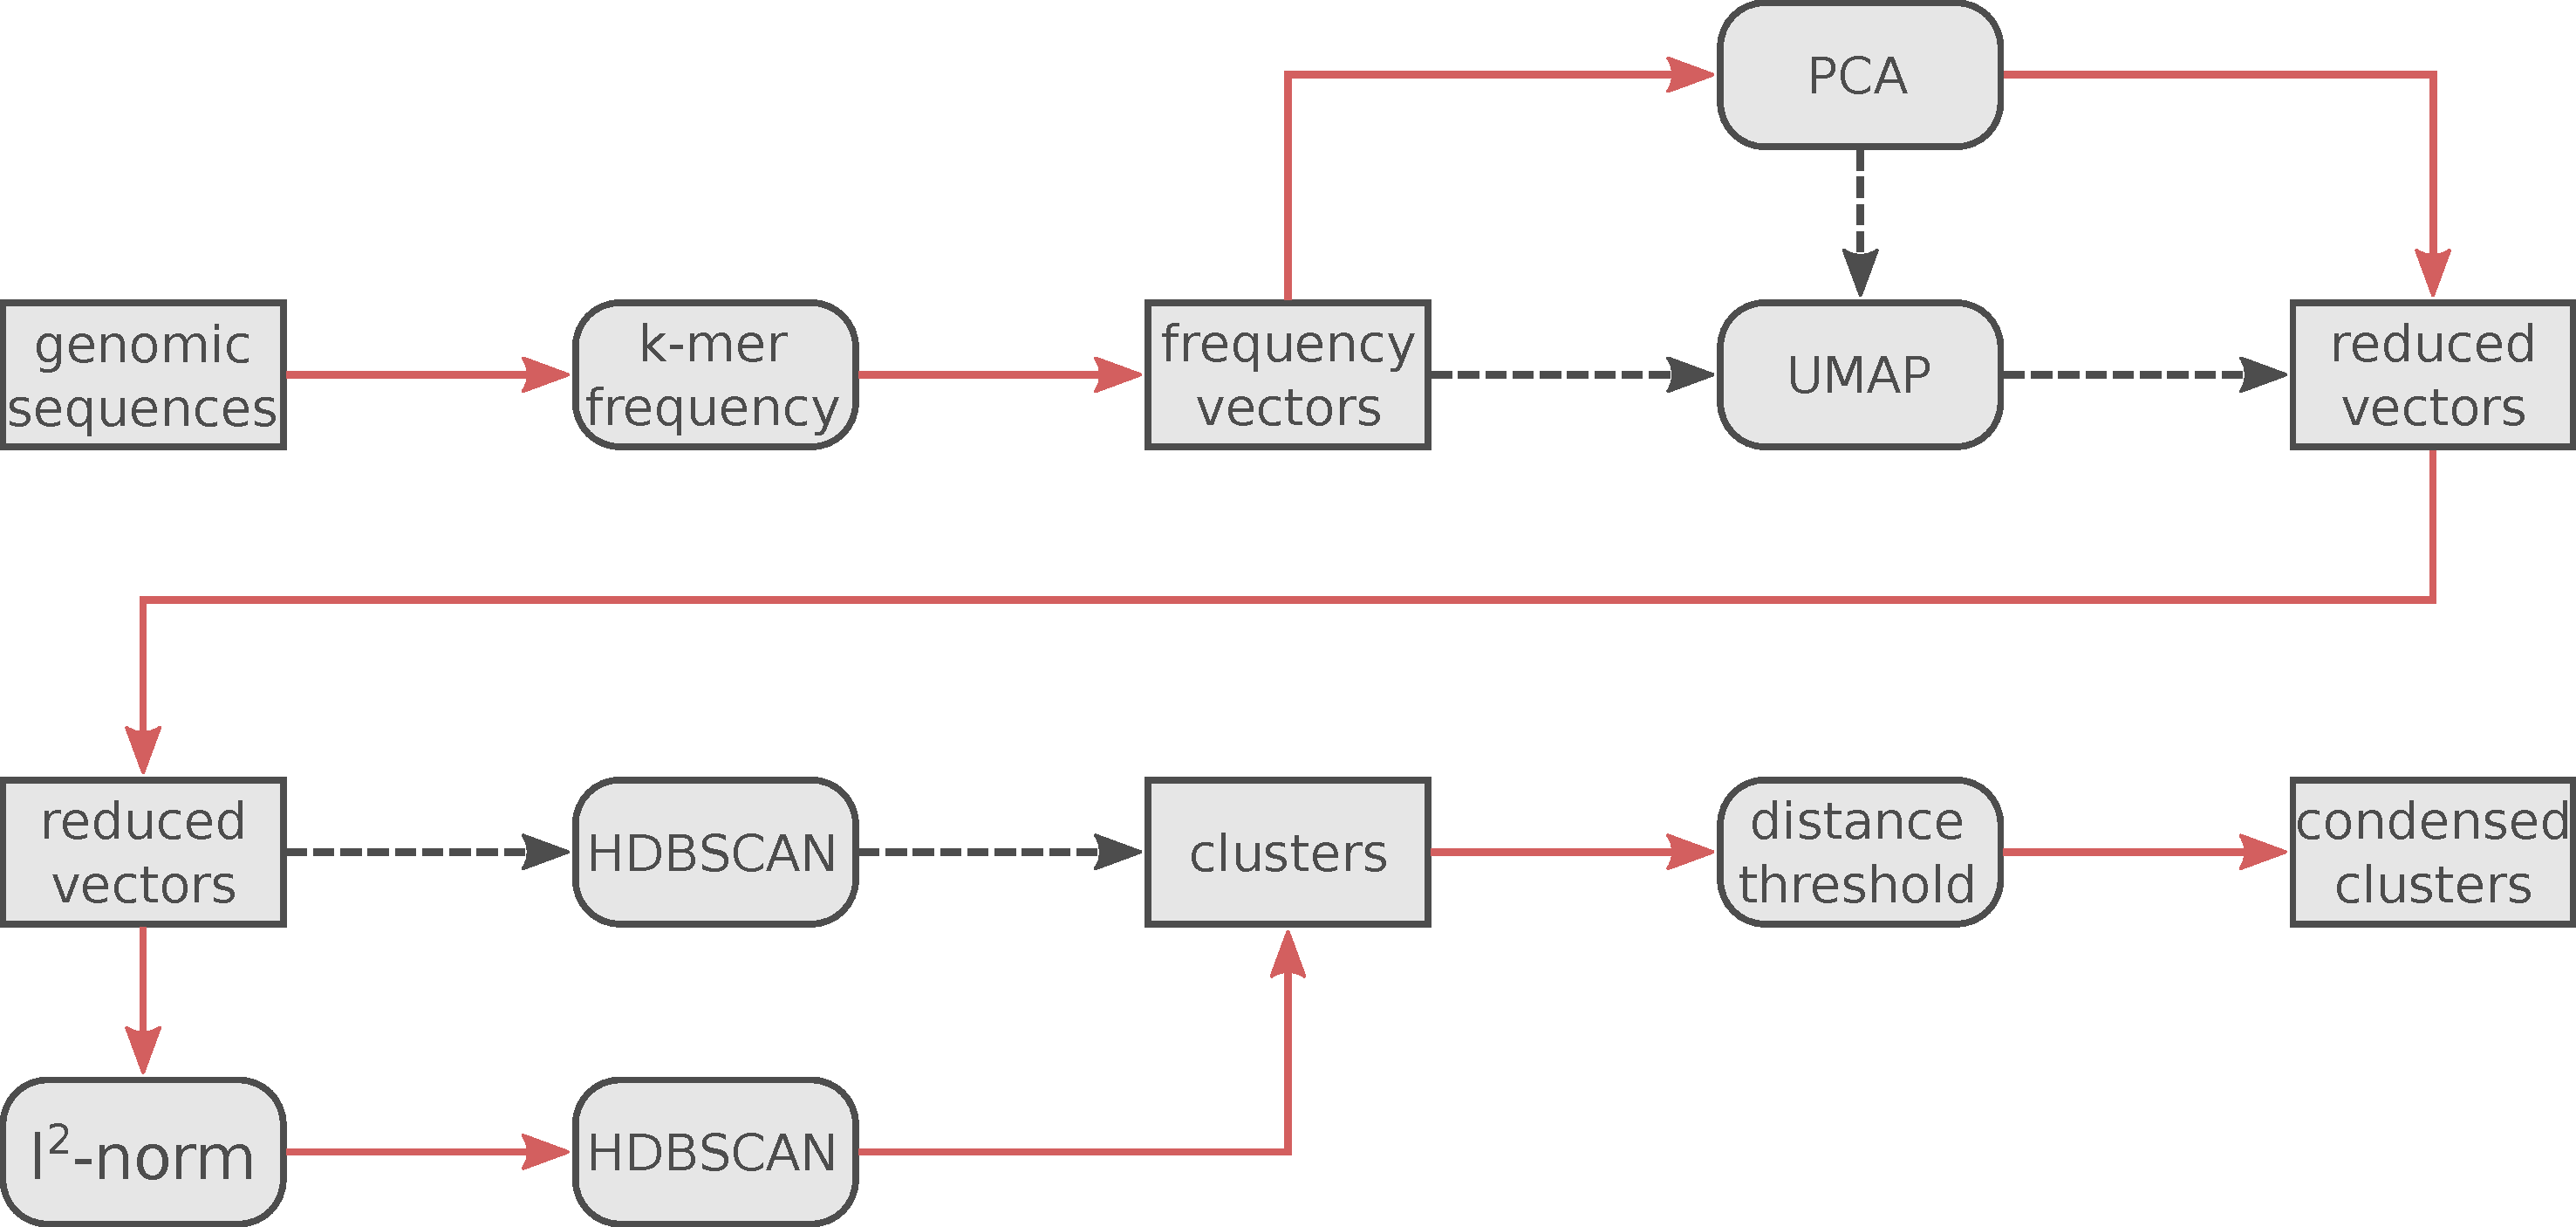
\includegraphics[width=\dimexpr\textwidth-2\fboxsep-2\fboxrule,fbox]{Graphics/Pipeline_V2.pdf}
    \caption[Clustering Pipeline]{\textbf{Clustering Pipeline.} .}
    \label{fig:Clustering_Pipeline}
\end{figure}

\begin{table}[!hbt]
    \centering
    \caption[Explained Variance by different PCA settings]{\textbf{Explained Variance by different PCA settings.}.}
    \label{tab:PCA_Dimension}
    \pgfplotstabletypeset[
        every head row/.style={
            before row={
                \toprule
            },
            after row={
                \midrule
            },
        },
        every last row/.style={
            after row={
                \bottomrule
            },
        },
        begin table=\begin{tabular*}{.5\textwidth},
        end table=\end{tabular*},
        columns={0,1},
        columns/0/.style={int detect, multicolumn names=l,column name=\textbf{\#Components}, column type=@{\extracolsep{\fill} }r},
        columns/1/.style={multicolumn names=l,column name=\textbf{Explained Variance}, column type=r}
    ]
    {Graphics/PCA.csv}
\end{table}